\documentclass[border=10pt]{standalone}
\usepackage[european]{circuitikz}
\begin{document}
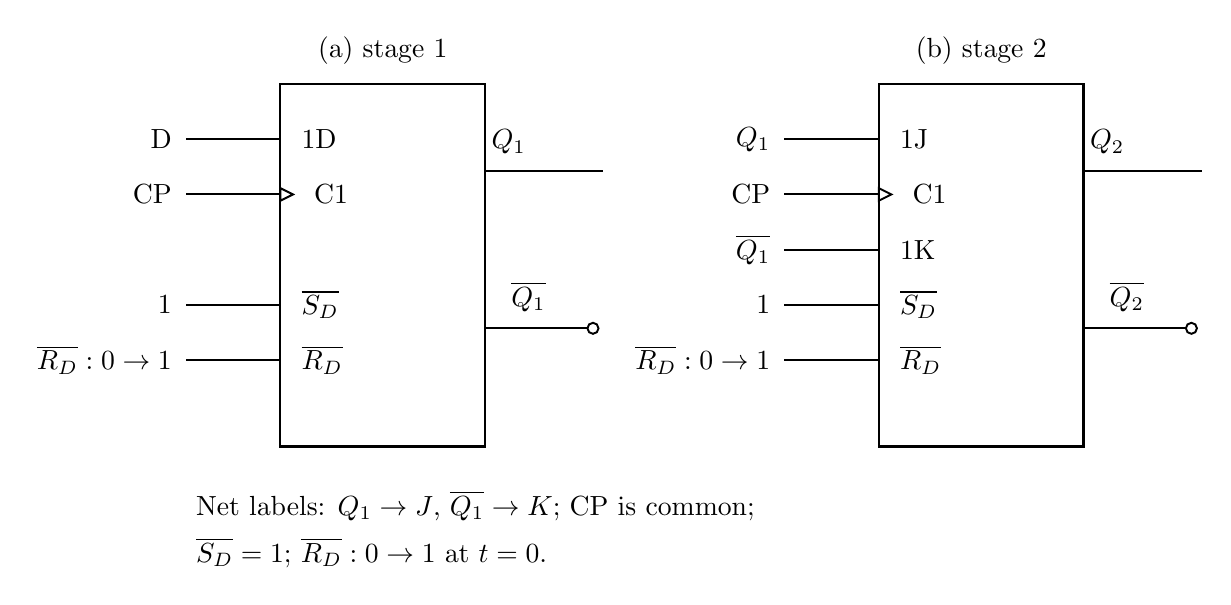
\begin{tikzpicture}[line width=0.7pt, font=\normalsize]

% 图 8.07：拆成两个独立子图，避免贯穿全图的长总线。
% 跨级连接用网标表达（Q1 -> J、Qbar1 -> K），CP 与 Rbar_D 也用网标，
% 不再画物理长线。数据严格照课程站 078 §3，不自行补条件。
% 框 2.6 x 4.6；输入行 3.9 / 3.2 / 2.5 / 1.8 / 1.1；输出行 3.5 / 1.5。
% 所有文字写在线的上方，线不穿框、不压字。

% 一个触发器级：#1 x 位移  #2 子图题  #3 数据端名  #4 数据端网标
%                #5 第二数据端名(空=D 型)  #6 第二数据端网标  #7 输出下标
\newcommand{\stage}[7]{%
  \begin{scope}[shift={(#1,0)}]
    \node[anchor=south] at (1.3,4.72) {#2};
    \draw[thick] (0,0) rectangle (2.6,4.6);
    \node[anchor=west] at (0.14,3.9) {#3};
    \draw (0,3.9) -- (-1.2,3.9);
    \node[anchor=east] at (-1.25,3.9) {#4};
    \node[anchor=west] at (0.3,3.2) {C1};
    \draw (0,3.12) -- (0,3.28) -- (0.16,3.2) -- cycle;
    \draw (0,3.2) -- (-1.2,3.2);
    \node[anchor=east] at (-1.25,3.2) {CP};
    \ifx\relax#5\relax\else
      \node[anchor=west] at (0.14,2.5) {#5};
      \draw (0,2.5) -- (-1.2,2.5);
      \node[anchor=east] at (-1.25,2.5) {#6};
    \fi
    \node[anchor=west] at (0.14,1.8) {$\overline{S_D}$};
    \draw (0,1.8) -- (-1.2,1.8);
    \node[anchor=east] at (-1.25,1.8) {1};
    \node[anchor=west] at (0.14,1.1) {$\overline{R_D}$};
    \draw (0,1.1) -- (-1.2,1.1);
    \node[anchor=east] at (-1.25,1.1) {$\overline{R_D}:0\to1$};
    \draw (2.6,3.5) -- (4.1,3.5);
    \node[anchor=south] at (2.9,3.58) {$Q_{#7}$};
    \draw (2.6,1.5) -- (3.9,1.5);
    \draw (3.97,1.5) circle (0.07);
    \node[anchor=south] at (3.15,1.58) {$\overline{Q_{#7}}$};
  \end{scope}
}

\stage{0}{(a) stage 1}{1D}{D}{\relax}{\relax}{1}
\stage{7.6}{(b) stage 2}{1J}{$Q_1$}{1K}{$\overline{Q_1}$}{2}

\node[anchor=west] at (-1.2,-0.75) {Net labels: $Q_1 \to J$, $\overline{Q_1} \to K$; CP is common;};
\node[anchor=west] at (-1.2,-1.35) {$\overline{S_D}=1$; $\overline{R_D}: 0 \to 1$ at $t=0$.};

\end{tikzpicture}
\end{document}
